\documentclass[a4paper,12pt]{article}
\usepackage[utf8]{inputenc}
\usepackage[T1]{fontenc}
\usepackage{lipsum}
\usepackage{enumitem}
\usepackage{geometry}
\geometry{margin=2.5cm}
\usepackage{graphicx}

\title{Práctica 1 Administracion de sistemas gestores de bases de datos}
\author{Alvaro Vazquez Vazquez}
\date{\today}

\usepackage{listings}
\usepackage{xcolor}

\lstset{
    basicstyle=\ttfamily,
    keywordstyle=\color{blue},
    stringstyle=\color{red},
    commentstyle=\color{green},
    showstringspaces=false,
    numbers=left,
    numberstyle=\tiny,
    frame=single,
    breaklines=true,
    morekeywords={firefox, ls, cd, echo}
}




\begin{document}
\maketitle

\noindent
I.E.S. Fernando Aguilar Quignon \\
C/Conil de la Frontera, 3 \\
CP 11010, Cádiz \\
\hrule

\section*{Despliegue del servidor delfos y exportación a Postgres}


\subsection{Intalacion de la maquina virtual}

Lo primero que debemos preparar es el sistema sobre el que va a correr nuestro servidor de bases de datos. Para ello, he optado por usar una maquina virtual con qemu/kvm. El sistema operativo sera un ubuntu server 24.04.3 LTS.






\subsubsection{Instalacion de qemu/kvm y virt-manager}

Para instalar y configurar qemu/kvm y virt-manager, he seguido los siguientes pasos en mi maquina host (Arch Linux):  


\begin{itemize}
    \item \textbf{sudo pacman -S install qemu-kvm libvirt-daemon-system libvirt-clients bridge-utils virt-manager} : Instalamos los paquetes necesarios para crear y gestionar maquinas virtuales.
    \item \textbf{sudo systemctl enable --now libvirtd} : Habilitamos el servicio de libvirt para que se inicie automaticamente al arrancar el sistema.
    \item \texttt{sudo usermod -aG libvirt \$(whoami)} : Añadimos nuestro usuario al grupo libvirt para poder gestionar las maquinas virtuales sin necesidad de permisos de superusuario.
    \item \textbf{newgrp libvirt} : Aplicamos los cambios de grupo sin necesidad de cerrar la sesión.
    \item \textbf{virt-manager} : Abrimos el gestor de maquinas virtuales.
\end{itemize}

\newpage

\subsubsection{Creacion de la maquina virtual en virt-manager}

\begin{figure}[h!]
    \centering
    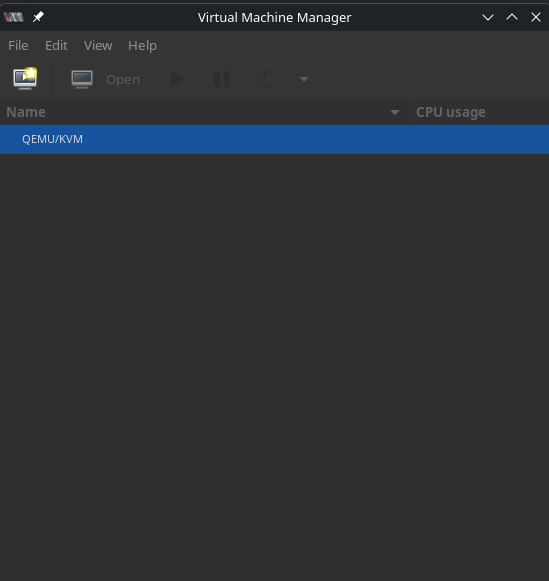
\includegraphics[width=0.5\textwidth]{1.png}
    \caption{Virtual Manager interface.}
\end{figure}

    \begin{itemize}
        \item Anadimos la imagen ISO de Ubuntu Server 24.04.3 LTS.
        \begin{figure}[h!]
        \centering
        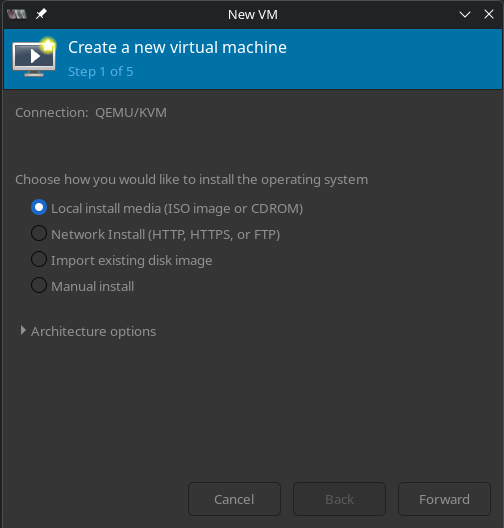
\includegraphics[width=0.5\textwidth]{2.png}
        \caption{Imagen ISO.}

    \end{figure}

    \begin{figure}[h!]
        \centering
        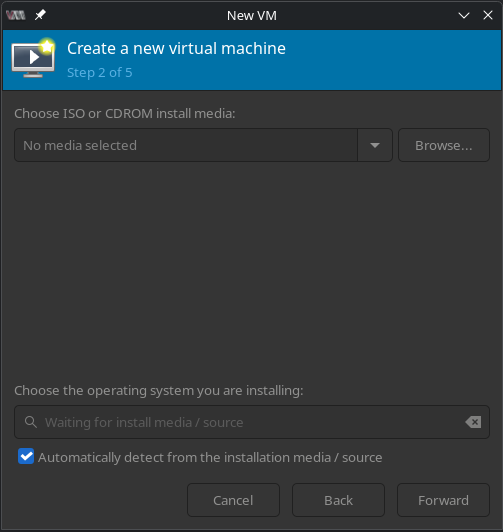
\includegraphics[width=0.5\textwidth]{3.png}
        \caption{ISO.}

    \end{figure}

    
    \begin{figure}[h!]
        \centering
        
\includegraphics[width=0.5\textwidth]{4.png}
        \caption{Imagen ISO.}

    \end{figure}

        \item Seleccionamos la cantidad de RAM y CPU que queremos asignar a la maquina virtual.
        
        
        \begin{figure}[h!]
            \centering
            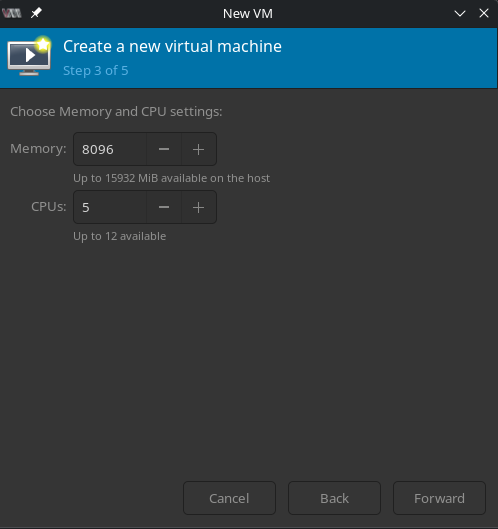
\includegraphics[width=0.5\textwidth]{5.png}
            \caption{Imagen ISO.}

        \end{figure}

        \item Creamos un disco duro virtual para la maquina virtual de 25GB.
        
        \begin{figure}[h!]
            \centering
            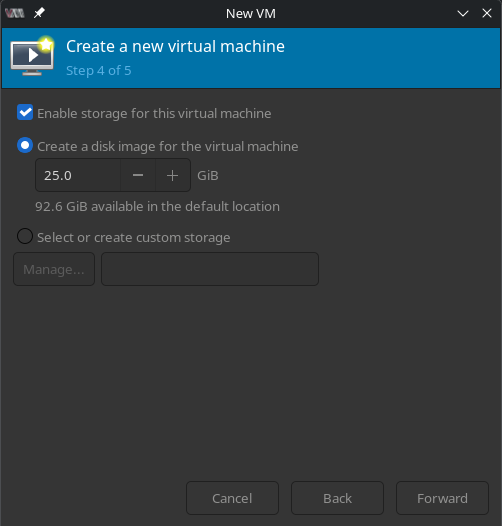
\includegraphics[width=0.5\textwidth]{6.png}
            \caption{Disco virtual.}
        \end{figure}
    
        \item Configuracion de red en modo puente (bridge) para que la maquina virtual tenga acceso a la red local y a internet.
    
        \begin{figure}[h!]
            \centering
            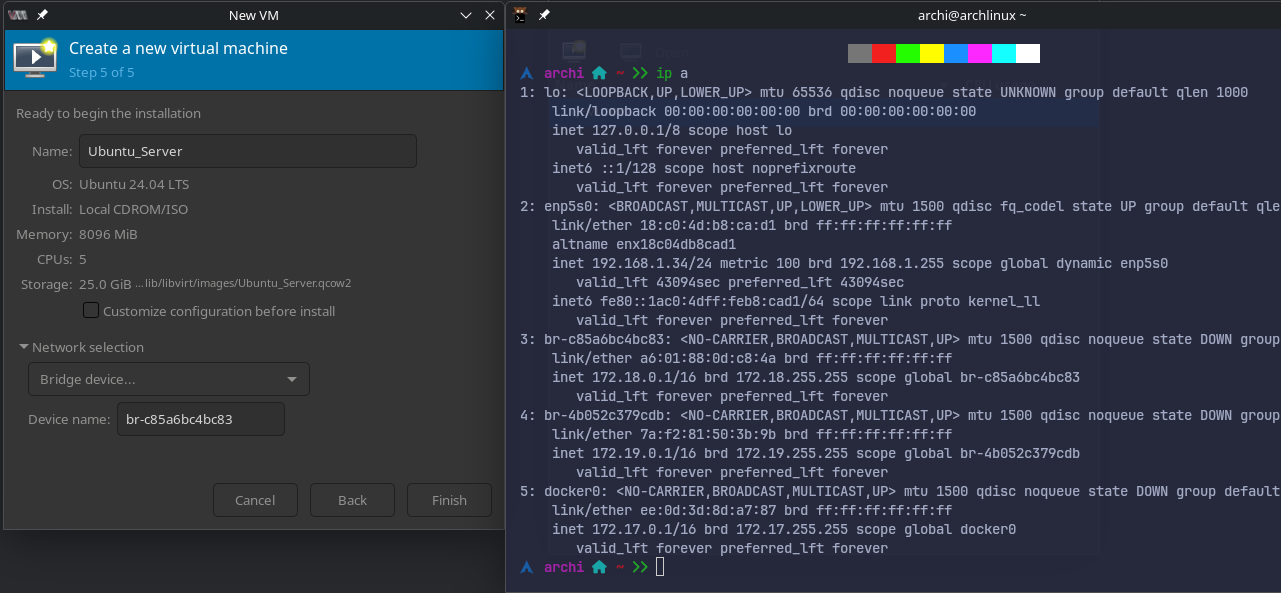
\includegraphics[width=1\textwidth]{7.png}
            \caption{Red en modo puente.}
        \end{figure}

    \subsubsection{Instalacion de Ubuntu Server 24.04.3 LTS}

    Iniciamos la maquina virtual y seguimos los pasos del instalador de Ubuntu Server 24.04.3 LTS.
    \newpage
    \begin{figure}[h!]
        \centering
        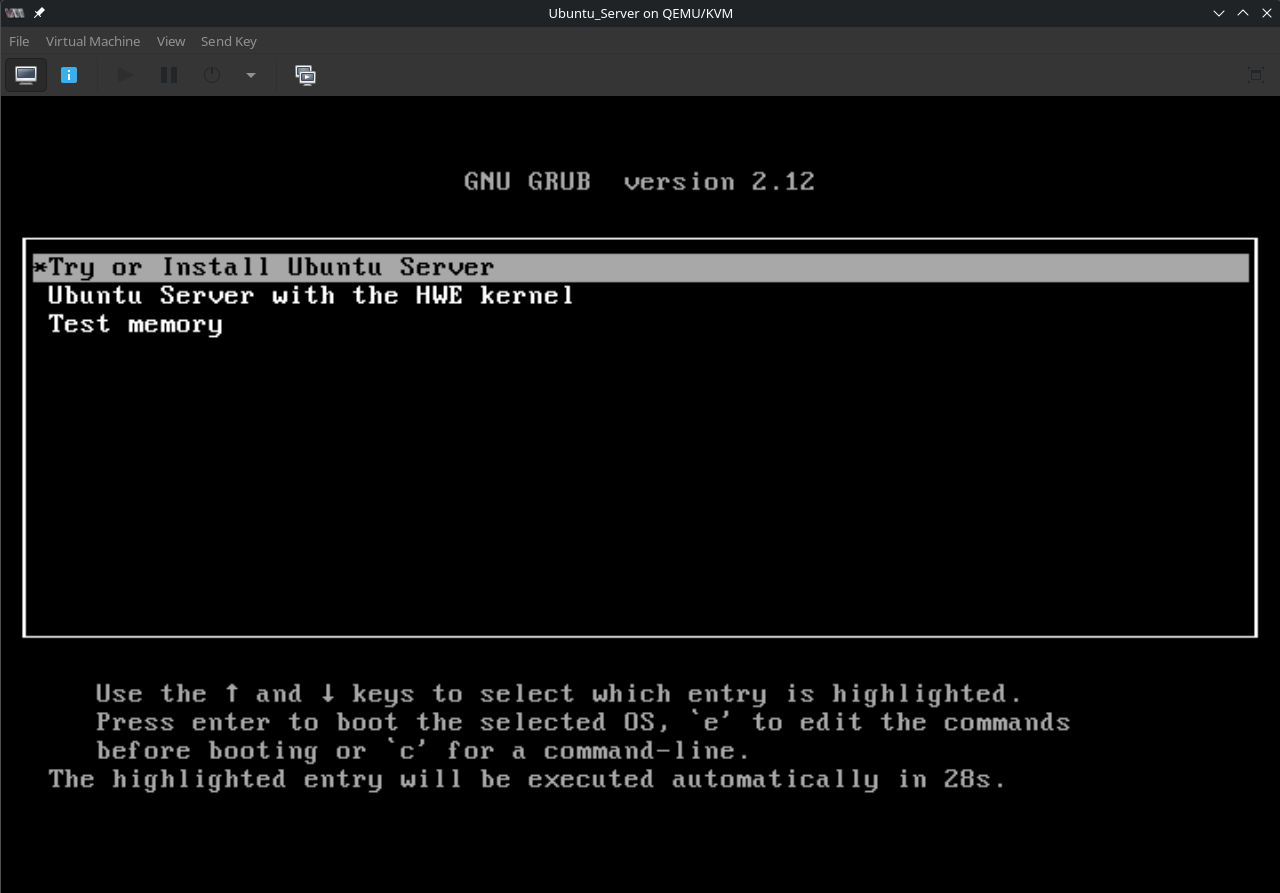
\includegraphics[width=0.5\textwidth]{8.png}
        \caption{Instalacion de Ubuntu Server.}
    \end{figure}

    \begin{figure}[h!]
        \centering
        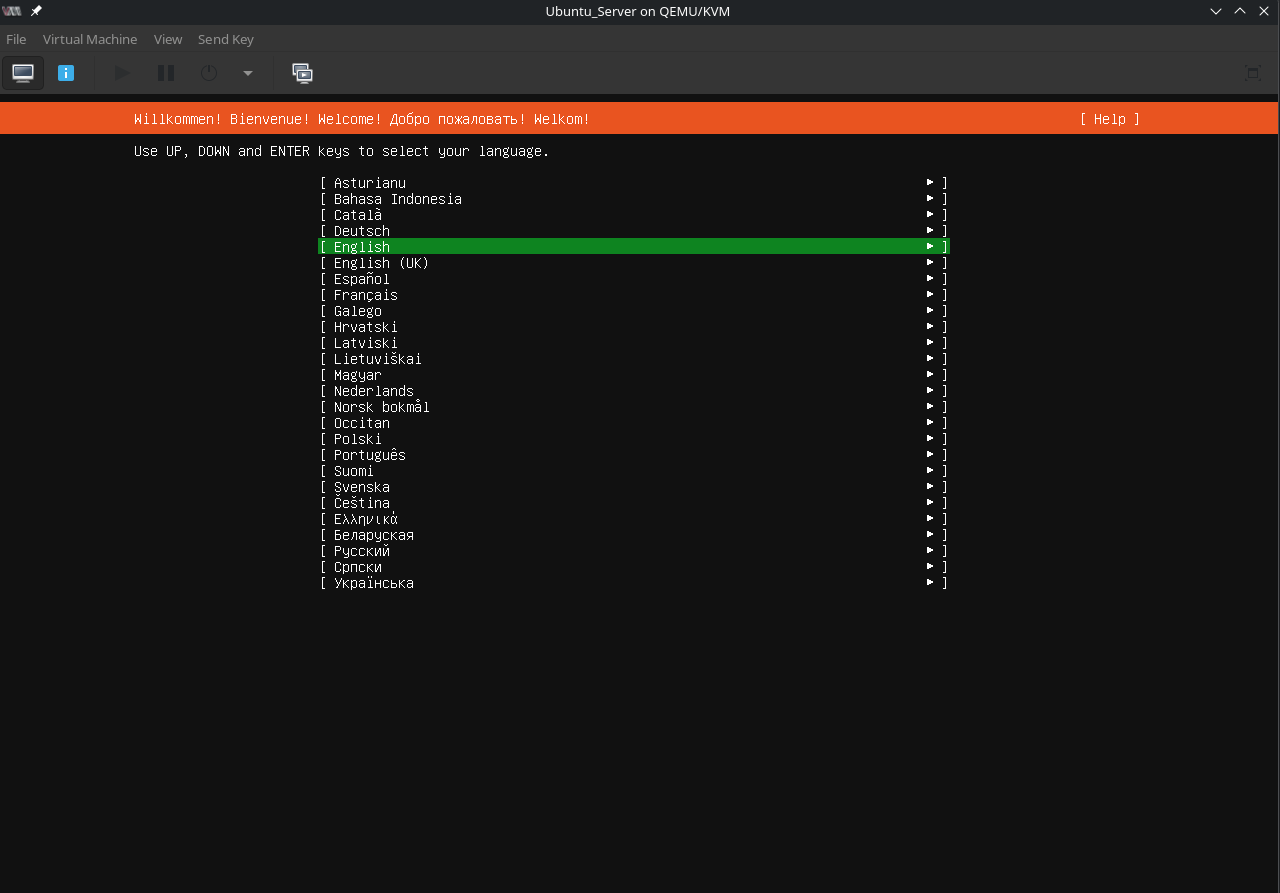
\includegraphics[width=0.5\textwidth]{9.png}
        \caption{Instalacion de Ubuntu Server.}
    \end{figure}

    \begin{figure}[h!]
        \centering
        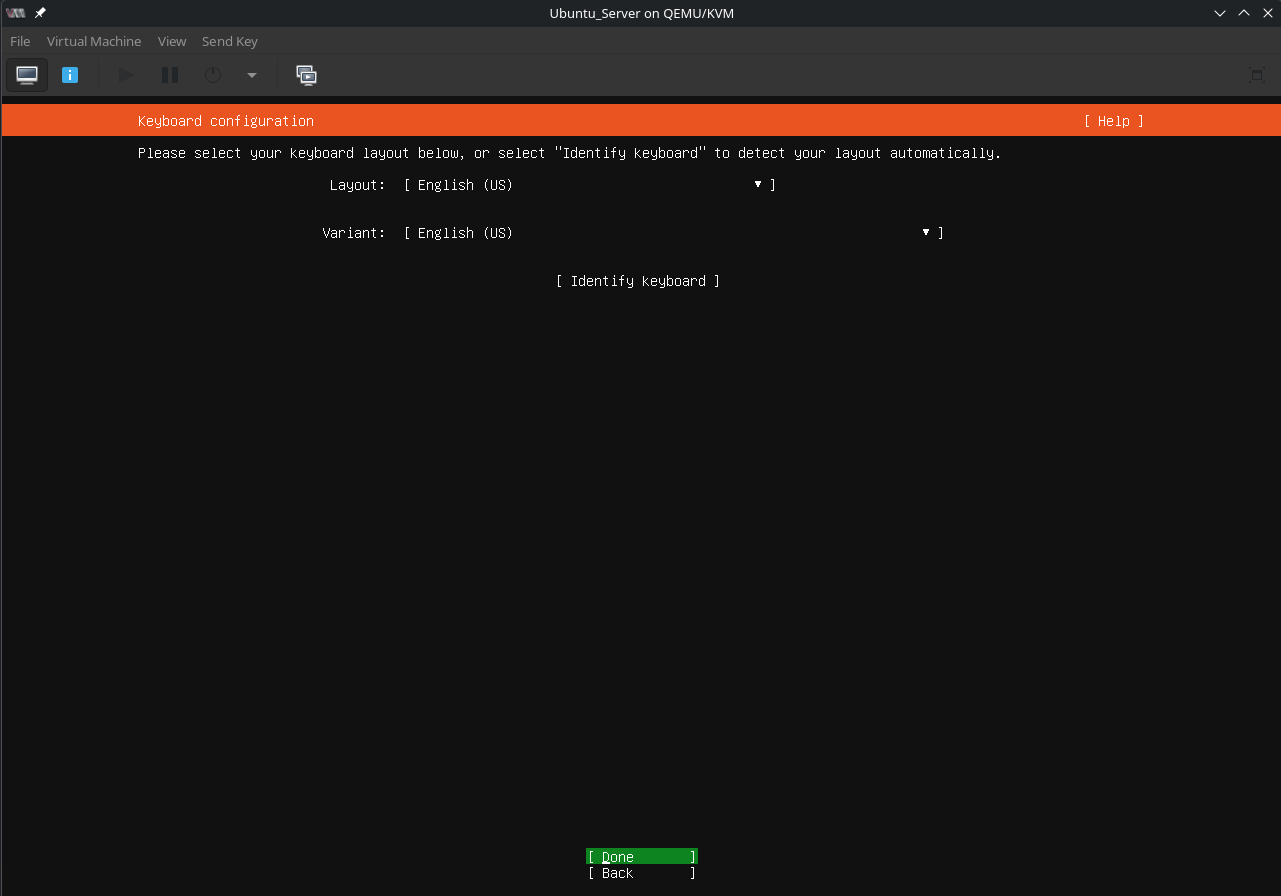
\includegraphics[width=0.5\textwidth]{10.png}
        \caption{Instalacion de Ubuntu Server.}
    \end{figure}
    \begin{figure}[h!]
        \centering
        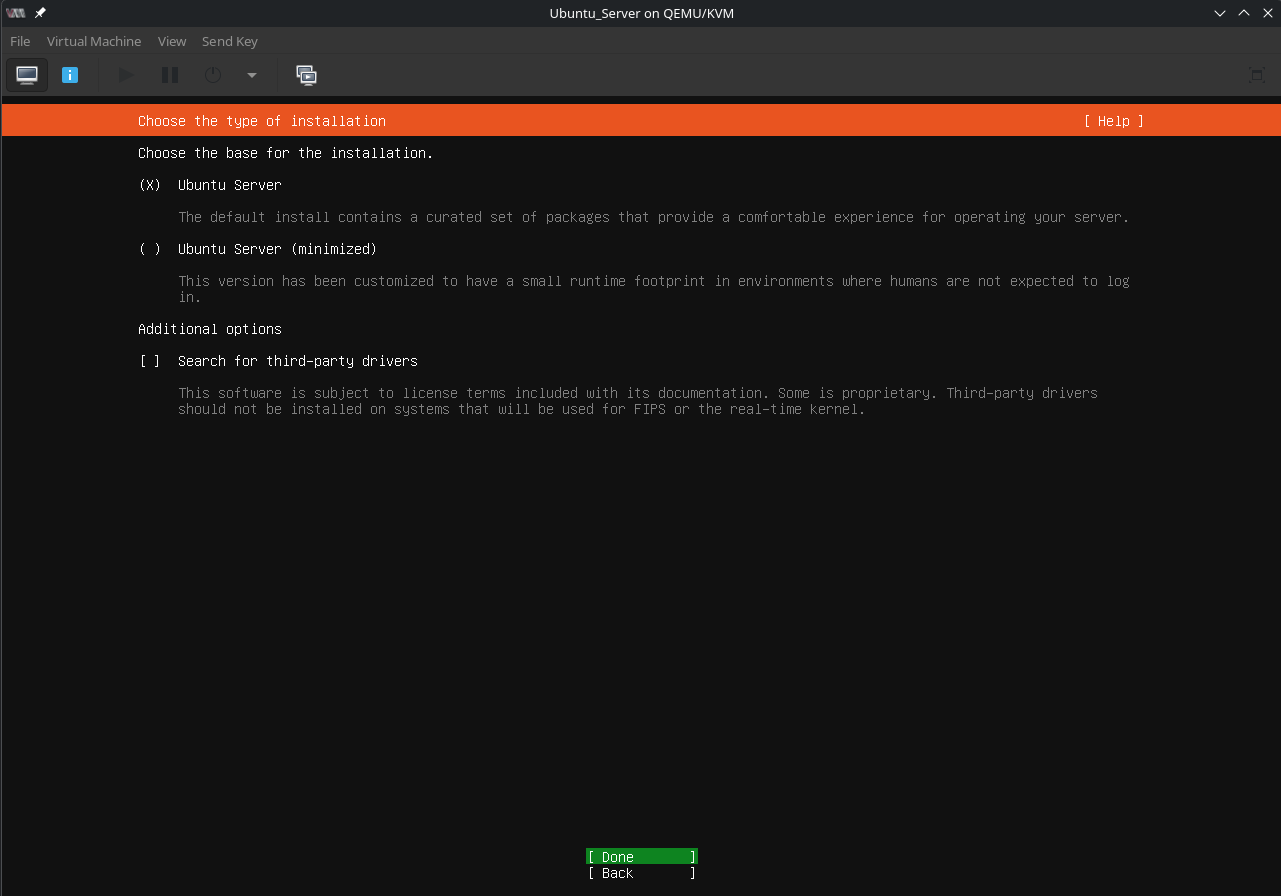
\includegraphics[width=0.5\textwidth]{11.png}
        \caption{Instalacion de Ubuntu Server.}
    \end{figure}
    \newpage
    \begin{figure}[h!]
        \centering
        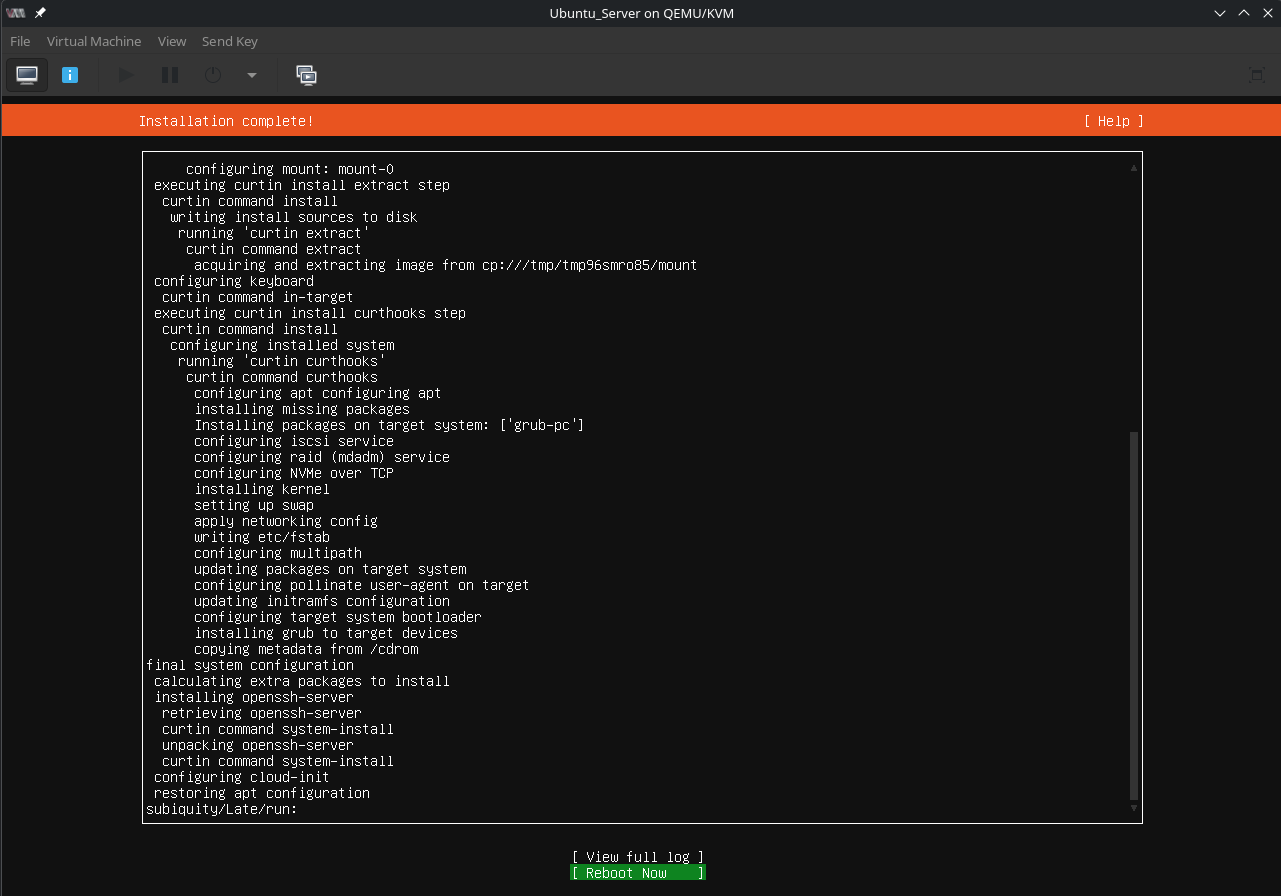
\includegraphics[width=0.5\textwidth]{12.png}
        \caption{Instalacion de Ubuntu Server.}
    \end{figure}

    \subsubsection{Configuracion inicial de la maquina virtual}

    \begin{figure}
        \centering
        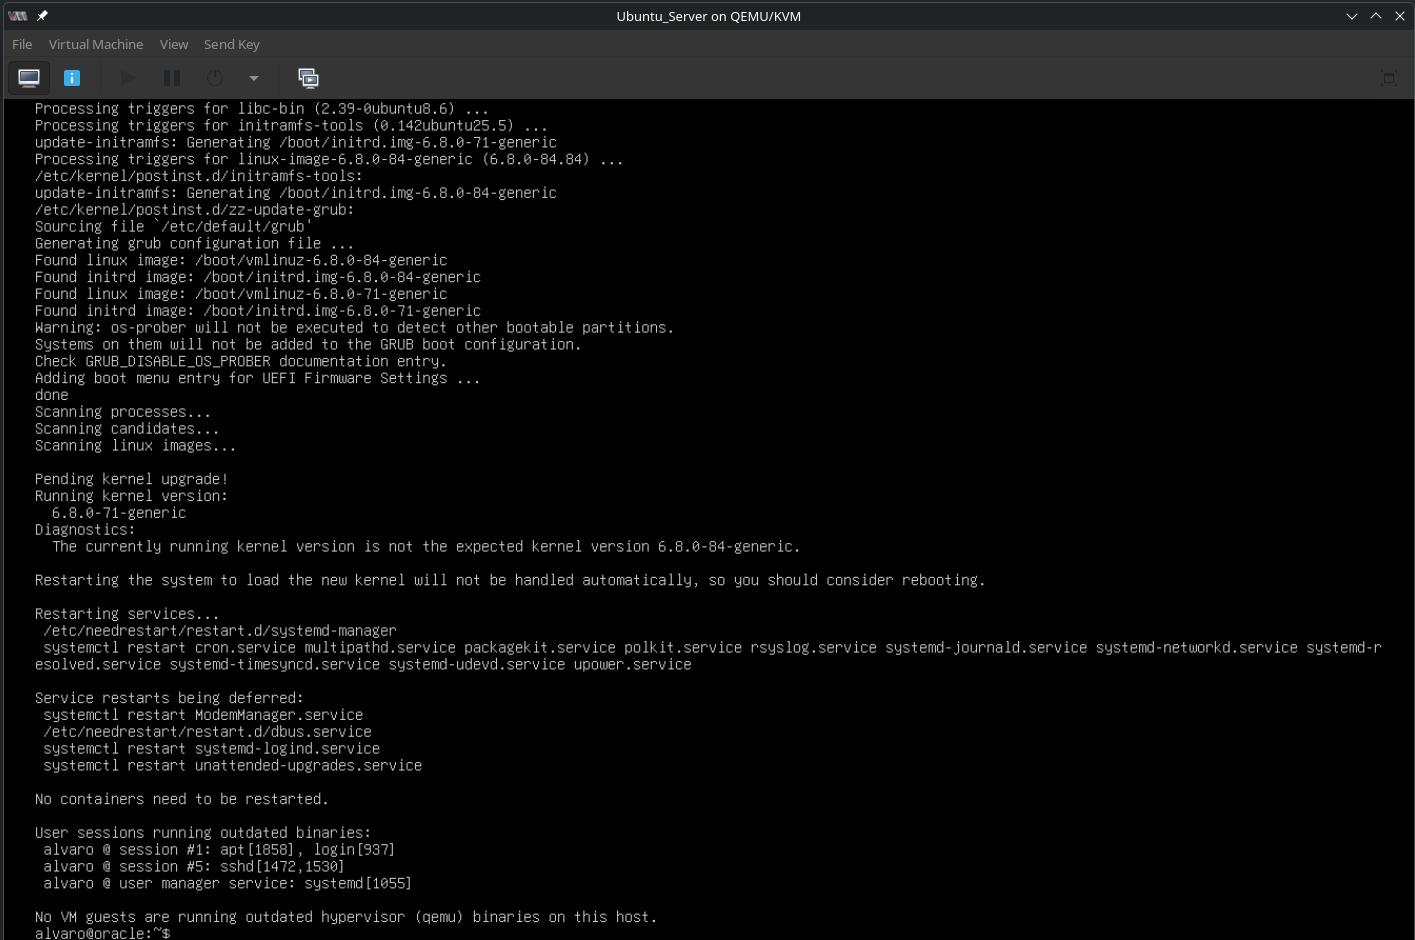
\includegraphics[width=0.5\textwidth]{13.png}
        \caption{Dentro de la maquina Ubuntu server.}
    \end{figure}

    \newpage

    \textbf{Es necesaria la configuracion del fichero /etc/netplan/00-installer-config.yaml para que la maquina virtual tenga una IP fija en la red local.}

    \begin{figure}[h!]
        \centering
        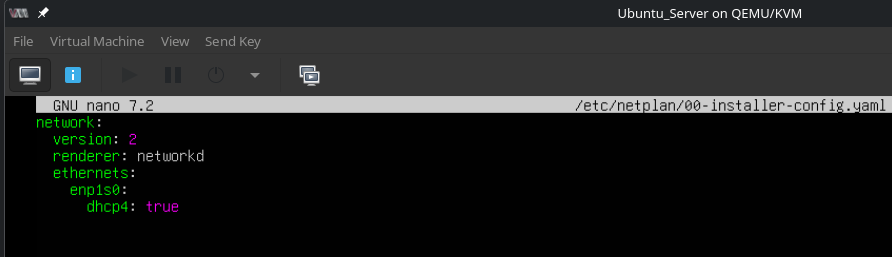
\includegraphics[width=0.5\textwidth]{14.png}
        \caption{Configuracion del fichero netplan.}
    \end{figure}


    \end{itemize}


\end{document}